\section{Introduction}

The main goal of this project is to implement control and trajectory architectures for bone surgeries, taking into account geometric, kinematic and dynamic models of planar robots.

\subsection{Contextualization}

The planar surgical robot represented in Fig. \ref{fig:enunciado} interacts with a virtual bone for surgery. The surgeon grabs directly the tip for operation (comanipulation mode), which should be done along a specific Cartesian direction. 

\begin{figure}[H]
    \centering
    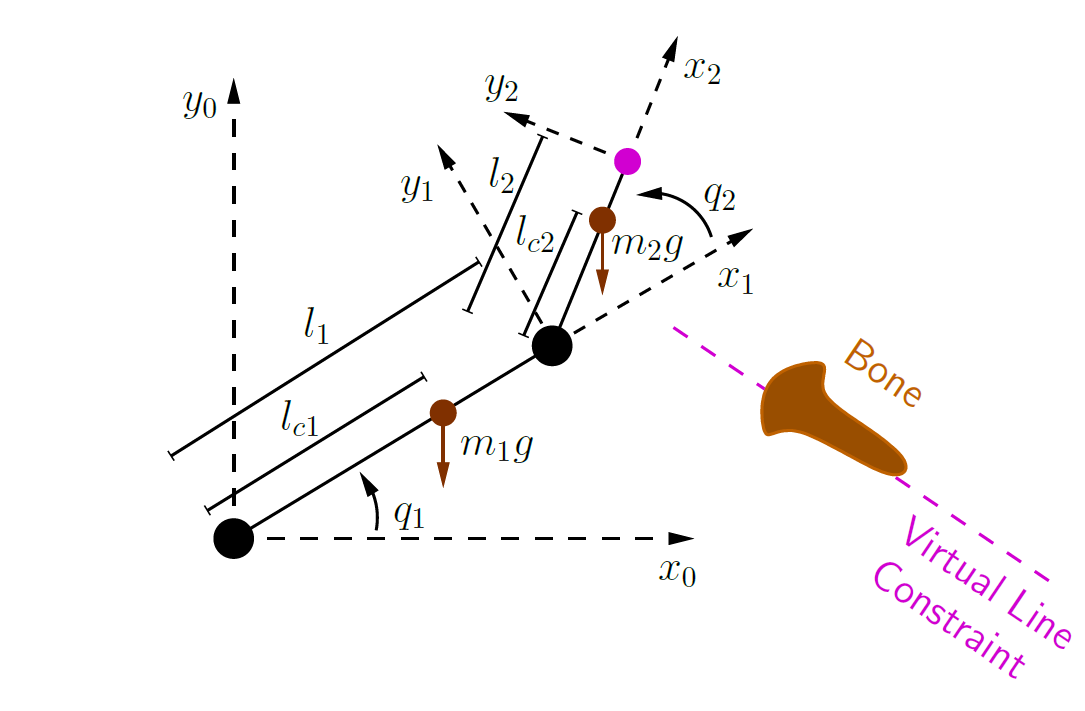
\includegraphics[width=0.49\textwidth]{imgs/foto_enunciado.png}
    \caption{Two-link planar robot for bone surgeries}
    \label{fig:enunciado}
\end{figure}































